%%% !TeX document-id = {7f856805-4d41-4d13-829b-b08b1a8ea49a}
 %%%  کلاس AUTthesis، نسخه اردیبهشت 1396
%%%   دانشگاه صنعتی امیرکبیر                 http://www.aut.ac.ir
%%%  تالار گفتگوی پارسی‌لاتک،       http://forum.parsilatex.com
%%%   آپدیت شده در آبان 95
%%      پشتیبانی و راهنمایی          badali_farhad@yahoo.com
%%%
%%%   بازبینی و اصلاح شده در اردیبهشت ماه 1396
%%%  Tested via TeXstudio in TeXlive 2014,‌‌ 2015 & 2016.
%%%

%-----------------------------------------------------------------------------------------------------
%        روش اجرا.: 2 بار F1 ، 2 بار  F11(به منظور تولید مراجع) ، دوبار Ctrl+Alt+I (به منظور تولید نمایه) و دو بار F1 -------> مشاهده Pdf
%%%%%%%%%%%%%%%%%%%%%%%%%%%%%%%%%%%%%%%%%%%%%%%%%%%%%%
%   TeXstudio as your IDE
%%  برای compile در TeXstudio تنها کافی است منوی Options->Configure TeXstudio را زده و در پنجره Configure TeXstudio در بخش Build گزینه Default Compiler را به XeLaTeX تغییر دهید. سند شما به راحتی compile خواهد شد.
%   F1 & F5 : Build & view
%   F6      : Compile
%   F7      : View
%   --------------
%   شما می‌توانید این نرم‌افزار را از سایت زیر دریافت کنید. برای استفاده از این نرم‌افزار باید پیش از نصب آن TeXlive را نصب کرده باشید.
%   TeXstudio.org
%   این سند با نسخه‌های 2014، 2015 و 2016 نرم‌افزار TeXlive در محیط TeXstudio آزمایش شده است.
%   نکته: در هنگام compile با نرم‌افزار TeXstudio فایل اصلی حتما باید باز باشد ولی نیازی نیست که روی tab آن باشید.
%	همچنین در پوشه LookAtMe فایلهای png برای راهنمایی وجود دارند.
%	برای ساخت میانبر نیم فاصله نیز به فایلهای پوشه LookAtMe را نگاه کنید.
%   باآرزوی پیروزی برای شما
%   آریا
%%%%%%%%%%%%%%%%%%%%%%%%%%%%%%%%%%%%%%%%%%%%%%%%%%%%%%
%        اگر قصد نوشتن رساله دکتری را دارید، در خط زیر به جای msc،
%      کلمه phd را قرار دهید. کلیه تنظیمات لازم، به طور خودکار، اعمال می‌شود.
%%% !TEX TS-program = XeLaTeX
\documentclass[oneside,bsc]{AUTthesis}
%       فایل commands.tex را حتماً به دقت مطالعه کنید؛ چون دستورات مربوط به فراخوانی بسته زی‌پرشین
%       و دیگر بسته‌ها و ... در این فایل قرار دارد و بهتر است که با نحوه استفاده از آنها آشنا شوید. توجه شود برای نسخه نهایی پایان‌نامه حتماً hyperref را
%        غیرفعال کنید.


% در این فایل، دستورها و تنظیمات مورد نیاز، آورده شده است.
%-------------------------------------------------------------------------------------------------------------------
% در ورژن جدید زی‌پرشین برای تایپ متن‌های ریاضی، این سه بسته، حتماً باید فراخوانی شود.
\usepackage{amsthm,amssymb,amsmath,amsfonts}
% بسته‌ای برای تنطیم حاشیه‌های بالا، پایین، چپ و راست صفحه
\usepackage[top=30mm, bottom=30mm, left=25mm, right=30mm]{geometry}
% بسته‌‌ای برای ظاهر شدن شکل‌ها و تصاویر متن
\usepackage{graphicx}
\usepackage{color}
\usepackage{todonotes}
%بسته‌ای برای تنظیم فاصله عمودی خط‌های متن
\usepackage{setspace}
\setstretch{1.3}
\usepackage{tocloft}
\renewcommand{\cftsecleader}{\cftdotfill{\cftdotsep}}
\usepackage{titleps}
\usepackage{titletoc}
\usepackage{tocloft}
\usepackage{multirow}
\usepackage{tabularx}
\usepackage{booktabs}
\usepackage{listings}
%با فعال کردن بسته زیر فوت‌نوت‌ها در هر صفحه ریست می‌شوند. حالت پیش‌فرض آن ریست شدن در هر فصل است
%\usepackage[perpage]{footmisc}
\usepackage{enumitem}
%\usepackage{titlesec}
% بسته‌ و دستوراتی برای ایجاد لینک‌های رنگی با امکان جهش
\usepackage[pagebackref=false,colorlinks,linkcolor=blue,citecolor=red]{hyperref}
\usepackage[nameinlink]{cleveref}%capitalize,,noabbrev
\AtBeginDocument{%
    \crefname{equation}{برابری}{equations}%
    \crefname{chapter}{فصل}{chapters}%
    \crefname{section}{بخش}{sections}%
    \crefname{appendix}{پیوست}{appendices}%
    \crefname{enumi}{مورد}{items}%
    \crefname{footnote}{زیرنویس}{footnotes}%
    \crefname{figure}{شکل}{figures}%
    \crefname{table}{جدول}{tables}%
    \crefname{theorem}{قضیه}{theorems}%
    \crefname{lemma}{لم}{lemmas}%
    \crefname{corollary}{نتیجه}{corollaries}%
    \crefname{proposition}{گزاره}{propositions}%
    \crefname{definition}{تعریف}{definitions}%
    \crefname{result}{نتیجه}{results}%
    \crefname{example}{مثال}{examples}%
    \crefname{remark}{نکته}{remarks}%
    \crefname{note}{یادداشت}{notes}%
}
% چنانچه قصد پرینت گرفتن نوشته خود را دارید، خط بالا را غیرفعال و  از دستور زیر استفاده کنید چون در صورت استفاده از دستور زیر‌‌،
% لینک‌ها به رنگ سیاه ظاهر خواهند شد که برای پرینت گرفتن، مناسب‌تر است
%\usepackage[pagebackref=false]{hyperref}
% بسته‌ لازم برای تنظیم سربرگ‌ها
\usepackage{fancyhdr}
% بسته‌ای برای ظاهر شدن «مراجع»  در فهرست مطالب
\usepackage[nottoc]{tocbibind}
% دستورات مربوط به ایجاد نمایه
\usepackage{makeidx,multicol}
\setlength{\columnsep}{1.5cm}
%\usepackage{tensor}
\usepackage[all]{xy}
\usepackage{tikz}
\usetikzlibrary{arrows}
%%%%%%%%%%%%%%%%%%%%%%%%%%
\usepackage{verbatim}
\makeindex
\usepackage{sectsty}
% فراخوانی بسته زی‌پرشین و تعریف قلم فارسی و انگلیسی
\usepackage[localise]{xepersian}%[extrafootnotefeatures]
\SepMark{-}

\setlatintextfont[
  Path=fonts/,
  UprightFont = *-Regular,
  BoldFont = *-Bold,
  ItalicFont = *-Italic
]{Neuton}

%حتماً از تک لایو 2014 استفاده کنید.
\settextfont[Scale=1.4,Path=fonts/]{BNazanin}
\renewcommand{\baselinestretch}{1.5}
\renewcommand{\labelitemi}{$\bullet$}
%%%%%%%%%%%%%%%%%%%%%%%%%%
% چنانچه می‌خواهید اعداد در فرمول‌ها، انگلیسی باشد، خط زیر را غیرفعال کنید.
%در غیر اینصورت حتماً فونت PGaramond را نصب کنید.
%\setdigitfont[Scale=1.1]{PGaramond}%%Yas
%%%%%%%%%%%%%%%%%%%%%%%%%%
% تعریف قلم‌های فارسی اضافی برای استفاده در بعضی از قسمت‌های متن
\defpersianfont\nastaliq[Scale=2,Path=fonts/]{IranNastaliq}
\defpersianfont\chapternumber[Scale=3,Path=fonts/]{BNazanin}
\chapterfont{\centering}%
%%%%%%%%%%%%%%%%%%%%%%%%%%
% دستوری برای تغییر نام کلمه «اثبات» به «برهان»
\renewcommand\proofname{\textbf{برهان}}

% دستوری برای تغییر نام کلمه «کتاب‌نامه» به «منابع و مراجع«
\renewcommand{\bibname}{منابع و مراجع}

\eqcommand{تارنما}{href}

% Headings for every page of ToC, LoF and Lot
\setlength{\cftbeforetoctitleskip}{-1.2em}
\setlength{\cftbeforelottitleskip}{-1.2em}
\setlength{\cftbeforeloftitleskip}{-1.2em}
\setlength{\cftaftertoctitleskip}{-1em}
\setlength{\cftafterlottitleskip}{-1em}
\setlength{\cftafterloftitleskip}{-1em}
%%\makeatletter
%%%%\renewcommand{\l@chapter}{\@dottedtocline{1}{1em\bfseries}{1em}}
%%%%\renewcommand{\l@section}{\@dottedtocline{2}{2em}{2em}}
%%%%\renewcommand{\l@subsection}{\@dottedtocline{3}{3em}{3em}}
%%%%\renewcommand{\l@subsubsection}{\@dottedtocline{4}{4em}{4em}}
%%%%\makeatother


\newcommand\tocheading{\par عنوان\hfill صفحه \par}
\newcommand\lofheading{\hspace*{.5cm}\figurename\hfill صفحه \par}
\newcommand\lotheading{\hspace*{.5cm}\tablename\hfill صفحه \par}

\renewcommand{\cftchapleader}{\cftdotfill{\cftdotsep}}
\renewcommand{\cfttoctitlefont}{\hspace*{\fill}\LARGE\bfseries}%\Large
\renewcommand{\cftaftertoctitle}{\hspace*{\fill}}
\renewcommand{\cftlottitlefont}{\hspace*{\fill}\LARGE\bfseries}%\Large
\renewcommand{\cftafterlottitle}{\hspace*{\fill}}
\renewcommand{\cftloftitlefont}{\hspace*{\fill}\LARGE\bfseries}
\renewcommand{\cftafterloftitle}{\hspace*{\fill}}

%%%%%%%%%%%%%%%%%%%%%%%%%%
% تعریف و نحوه ظاهر شدن عنوان قضیه‌ها، تعریف‌ها، مثال‌ها و ...
%برای شماره گذاری سه تایی قضیه ها
\theoremstyle{definition}
\newtheorem{definition}{تعریف}[section]
\newtheorem{remark}[definition]{نکته}
\newtheorem{note}[definition]{یادداشت}
\newtheorem{example}[definition]{نمونه}
\newtheorem{question}[definition]{سوال}
\newtheorem{remember}[definition]{یاداوری}
\theoremstyle{theorem}
\newtheorem{theorem}[definition]{قضیه}
\newtheorem{lemma}[definition]{لم}
\newtheorem{proposition}[definition]{گزاره}
\newtheorem{corollary}[definition]{نتیجه}
%%%%%%%%%%%%%%%%%%%%%%%%
%%%%%%%%%%%%%%%%%%%
%%% برای شماره گذاری چهارتایی قضیه ها و ...
%%\newtheorem{definition1}[subsubsection]{تعریف}
%%\newtheorem{theorem1}[subsubsection]{قضیه}
%%\newtheorem{lemma1}[subsubsection]{لم}
%%\newtheorem{proposition1}[subsubsection]{گزاره}
%%\newtheorem{corollary1}[subsubsection]{نتیجه}
%%\newtheorem{remark1}[subsubsection]{نکته}
%%\newtheorem{example1}[subsubsection]{مثال}
%%\newtheorem{question1}[subsubsection]{سوال}

%%%%%%%%%%%%%%%%%%%%%%%%%%%%

% دستورهایی برای سفارشی کردن صفحات اول فصل‌ها
\makeatletter
\newcommand\mycustomraggedright{%
 \if@RTL\raggedleft%
 \else\raggedright%
 \fi}
\def\@makechapterhead#1{%
\thispagestyle{style1}
\vspace*{20\p@}%
{\parindent \z@ \mycustomraggedright %\@mycustomfont
\ifnum \c@secnumdepth >\m@ne
\if@mainmatter

\bfseries{\Huge \@chapapp}\small\space {\chapternumber\thechapter}
\par\nobreak
\vskip 0\p@
\fi
\fi
\interlinepenalty\@M
\Huge \bfseries #1\par\nobreak
\vskip 120\p@

}

%\thispagestyle{empty}
\newpage}
\bidi@patchcmd{\@makechapterhead}{\thechapter}{\tartibi{chapter}}{}{}
\bidi@patchcmd{\chaptermark}{\thechapter}{\tartibi{chapter}}{}{}
\makeatother

\pagestyle{fancy}
\renewcommand{\chaptermark}[1]{\markboth{\chaptername~\tartibi{chapter}: #1}{}}

\fancypagestyle{style1}{
\fancyhf{}
\fancyfoot[c]{\thepage}
\fancyhead[R]{\leftmark}%
\renewcommand{\headrulewidth}{1.2pt}
}


\fancypagestyle{style2}{
\fancyhf{}
\fancyhead[R]{چکیده}
\fancyfoot[C]{\thepage{}}
\renewcommand{\headrulewidth}{1.2pt}
}

\fancypagestyle{style3}{%
  \fancyhf{}%
  \fancyhead[R]{فهرست نمادها}
  \fancyfoot[C]{\thepage}%
  \renewcommand{\headrulewidth}{1.2pt}%
}

\fancypagestyle{style4}{%
  \fancyhf{}%
  \fancyhead[R]{فهرست جداول}
  \fancyfoot[C]{\thepage}%
  \renewcommand{\headrulewidth}{1.2pt}%
}

\fancypagestyle{style5}{%
  \fancyhf{}%
  \fancyhead[R]{فهرست اشکال}
  \fancyfoot[C]{\thepage}%
  \renewcommand{\headrulewidth}{1.2pt}%
}

\fancypagestyle{style6}{%
  \fancyhf{}%
  \fancyhead[R]{فهرست مطالب}
  \fancyfoot[C]{\thepage}%
  \renewcommand{\headrulewidth}{1.2pt}%
}

\fancypagestyle{style7}{%
  \fancyhf{}%
  \fancyhead[R]{نمایه}
  \fancyfoot[C]{\thepage}%
  \renewcommand{\headrulewidth}{1.2pt}%
}

\fancypagestyle{style8}{%
  \fancyhf{}%
  \fancyhead[R]{منابع و مراجع}
  \fancyfoot[C]{\thepage}%
  \renewcommand{\headrulewidth}{1.2pt}%
}
\fancypagestyle{style9}{%
  \fancyhf{}%
  \fancyhead[R]{واژه‌نامه‌ی فارسی به انگلیسی}
  \fancyfoot[C]{\thepage}%
  \renewcommand{\headrulewidth}{1.2pt}%
}
%


%دستور حذف نام لیست تصاویر و لیست جداول از فهرست مطالب
\newcommand*{\BeginNoToc}{%
  \addtocontents{toc}{%
    \edef\protect\SavedTocDepth{\protect\the\protect\value{tocdepth}}%
  }%
  \addtocontents{toc}{%
    \protect\setcounter{tocdepth}{-10}%
  }%
}
\newcommand*{\EndNoToc}{%
  \addtocontents{toc}{%
    \protect\setcounter{tocdepth}{\protect\SavedTocDepth}%
  }%
}
\newcounter{savepage}
\renewcommand{\listfigurename}{فهرست اشکال}
\renewcommand{\listtablename}{فهرست جداول}
%\renewcommand\cftsecleader{\cftdotfill{\cftdotsep}}
%%%%%%%%%%%%%%%%%%%%%%%%%%%%%
%%%%%%%%%%%%%%%%%%%%%%%%%%%%


\begin{document}
\baselineskip=.75cm
%% -!TEX root = AUTthesis.tex
% در این فایل، عنوان پایان‌نامه، مشخصات خود، متن تقدیمی‌، ستایش، سپاس‌گزاری و چکیده پایان‌نامه را به فارسی، وارد کنید.
% توجه داشته باشید که جدول حاوی مشخصات پروژه/پایان‌نامه/رساله و همچنین، مشخصات داخل آن، به طور خودکار، درج می‌شود.
%%%%%%%%%%%%%%%%%%%%%%%%%%%%%%%%%%%%
% دانشکده، آموزشکده و یا پژوهشکده  خود را وارد کنید
\faculty{دانشکده مهندسی کامپیوتر}
% گرایش و گروه آموزشی خود را وارد کنید
\department{}
% عنوان پایان‌نامه را وارد کنید
\fatitle{طراحي و پياده سازي سيستم پيش‌بينی ترافيک بر پايه شبکه‌های عصبی}
% نام استاد(ان) راهنما را وارد کنید
\firstsupervisor{دکتر رضا صفابخش}
%\secondsupervisor{استاد راهنمای دوم}
% نام استاد(دان) مشاور را وارد کنید. چنانچه استاد مشاور ندارید، دستور پایین را غیرفعال کنید.
% \firstadvisor{نام کامل استاد مشاور}
%\secondadvisor{استاد مشاور دوم}
% نام نویسنده را وارد کنید
\name{الهه}
% نام خانوادگی نویسنده را وارد کنید
\surname{داستان}
%%%%%%%%%%%%%%%%%%%%%%%%%%%%%%%%%%
\thesisdate{زمستان ۱۴۰۰}

% چکیده پایان‌نامه را وارد کنید
\fa-abstract{
پیش‌بینی سرعت ترافیک برای کنترل و هدایت آن ضروری است.
به علت پیچیدگی و غیرخطی بودن سرعت ترافیک روش‌های قدیمی نمی‌توانند ترافیک را برای سفرهایی با زمان طولانی و متوسط به خوبی پیش‌بینی کنند.
پیش‌بینی دقیق و بی‌درنگ سرعت ترافیک برای افراد و سازمان‌های ارائه دهنده‌ی خدمات حمل و نقل و حتی دولت موضوع مهمی است چرا که حمل و نقل نقش مهمی در زندگی هر فرد ایفا می‌کند و یکی از اصلی‌ترین توانایی‌ها در سیستم ترابری هوشمند \پانویس{Intelligent Transportation System} به شمار می‌رود.
در این پروژه سعی داریم با استفاده از آموزش دادن شبکه‌های عصبی عمیق به پیش‌بینی سرعت ترافیک در برخی نقاط مشخص (مانند چهارراه‌ها و میدان‌ها) بپردازیم.
امروزه با استفاده از داده‌های عظیمی که در دسترس است و همچنین پیشرفت سخت‌افزار می‌توانیم شبکه‌های عمیقی که در گذشته قابل آموزش نبودند را آموزش دهیم و از توانایی بالای آن‌ها در پیش بینی مسائل پیچیده استفاده کنیم. در این گزارش شبکه‌ی پیچشی گرافی زمانی-مکانی را برای پیش‌بینی سرعت ترافیک به کار گرفتیم و با استفاده از نتایج ارزیابی این مدل بر روی دو مجموعه‌داده‌ی واقعی نشان دادیم که این شبکه‌ی عمیق به طور موثری می‌تواند همبستگی‌های زمانی-مکانی جامع را درک کند و درنتیجه عملکرد خوبی از خود نشان دهد.
}

% کلمات کلیدی پایان‌نامه را وارد کنید
\keywords{
حمل و نقل، پیش‌بینی سرعت ترافیک، شبکه‌های عصبی عمیق
}



\AUTtitle
%%%%%%%%%%%%%%%%%%%%%%%%%%%%%%%%%%

\vspace*{7cm}
\thispagestyle{empty}
\begin{center}

\includegraphics[height=5cm,width=12cm]{images/in-the-name-of-god}
\end{center}
% تاییدیه دفاع
\newpage
\thispagestyle{empty}
%\fontsize{18pt}{19pt}\selectfont

\section*{صفحه فرم ارزیابی و تصویب پایان نامه- فرم تأیید اعضاء كميته دفاع}

\fontsize{12pt}{14pt}\selectfont
\renewcommand{\baselinestretch}{1.5}
\vspace*{1cm}
   در این صفحه فرم دفاع یا تایید و تصویب پایان نامه موسوم به فرم کمیته دفاع- موجود در پرونده آموزشی- را قرار دهید.
\vspace*{1cm}


\subsection*{نکات مهم:}
 
\begin{itemize}
\item
	نگارش پایان نامه/رساله باید به
	{\color{red}
		زبان فارسی
	}
	و بر اساس آخرین نسخه دستورالعمل و راهنمای تدوین پایان نامه های دانشگاه صنعتی امیرکبیر باشد.(دستورالعمل و راهنمای حاضر)
\item رنگ جلد پایان نامه/رساله چاپي كارشناسي، كارشناسي ارشد و دكترا  بايد به ترتيب مشكي، طوسي و سفيد رنگ باشد.  
\item چاپ و صحافی پایان نامه/رساله بصورت
{\color{red}
	پشت و رو(دورو)
}
بلامانع است و انجام آن توصيه مي شود. 
\end{itemize}
%%%%%%%%%%%%%%%%%%%%%%%%%%%%%%%%%%%%%%%%%%%%%%%%%%%%%%%%%%%%%%%%%%%%%%%%%%%%%%%%%%%%%%%%%%%%%%%%%%
%%%%%%%%%%%%%%%%%%%%%%%%%%%%%%%%%%%%%%%%%%%%%%%%%%%%%%%%%%%%%%%%%%%%%%%%%%%%%%%%%%%%%%%%%%%%%%%%%%
\newpage
\thispagestyle{empty}
\begin{picture}(50,50)
  \put(10,0){
\includegraphics[scale=.06]{images/fa-logo}}
  \put(4.5,-13){\footnotesize{دانشگاه صنعتی امیرکبیر}}
  \put(10.5,-27){\footnotesize{(پلی‌تکنیک تهران)}}
  \put(170,30){\bf{به نام خدا}}
  \put(140,-5){\Large\bf{تعهدنامه اصالت اثر}}
  \put(300,0){تاریخ: \datethesis}
\end{picture}

\vspace*{2.5cm}

اينجانب {\bf{\fname\ \lname}} متعهد می‌شوم که مطالب مندرج در این پایان‌نامه حاصل کار پژوهشی اینجانب تحت نظارت و راهنمایی اساتید دانشگاه صنعتی امیرکبیر بوده و به دستاوردهای دیگران که در این پژوهش از آنها استفاده شده است مطابق مقررات و روال متعارف ارجاع و در فهرست منابع و مآخذ ذکر گردیده است. این پایان‌نامه قبلاً برای احراز هیچ مدرک هم‌سطح یا بالاتر ارائه نگردیده است.

در صورت اثبات تخلف در هر زمان، مدرک تحصیلی صادر شده توسط دانشگاه از درجه اعتبار ساقط بوده و دانشگاه حق پیگیری قانونی خواهد داشت.


کلیه نتایج و حقوق حاصل از این پایان‌نامه متعلق به دانشگاه صنعتی امیرکبیر می‌باشد. هرگونه استفاده از نتایج علمی و عملی، واگذاری اطلاعات به دیگران یا چاپ و تکثیر، نسخه‌برداری، ترجمه و اقتباس از این پایان نامه بدون موافقت کتبی دانشگاه صنعتی امیرکبیر ممنوع است. 
نقل مطالب با ذکر مآخذ بلامانع است.\\
\vspace{2.5cm}


{\centerline {\bf{\fname\ \lname}}}
\vspace*{.2cm}
{\centerline{امضا}}
%%%%%%%%%%%%%%%%%%%%%%%%%%%%%%%%%
% چنانچه مایل به چاپ صفحات «تقدیم»، «نیایش» و «سپاس‌گزاری» در خروجی نیستید، خط‌های زیر را با گذاشتن ٪  در ابتدای آنها غیرفعال کنید.
% پایان‌نامه خود را تقدیم کنید
% نیایش خود را در فایل زیر بنویسید.
\begin{acknowledgementpage}

\vspace{1.5cm}

{\nastaliq
{}}\end{acknowledgementpage}
\newpage
%سپاسگزاری را در فایل زیر بنویسید.
%%%%%%%%%%%%%%%%%%%%%%%%%%%%%%%%%%%%%%%%%
%%%%%%%%%%%%%%%%%%%%%%%%%%%%%%%%%کدهای زیر را تغییر ندهید.
\newpage\clearpage

\pagestyle{style2}

\vspace*{-1cm}
\section*{\centering چکیده}
%\addcontentsline{toc}{chapter}{چکیده}
\vspace*{.5cm}
\ffa-abstract
\vspace*{2cm}


{\noindent\large\textbf{واژه‌های کلیدی:}}\par
\vspace*{.5cm}
\fkeywords

%دستور زیر برای شماره گذاری صفحات قبل از فصل اول با حروف ابجد است.
\pagenumbering{alph}
%-----------------------------------------------------------------------------
%در فایل زیر دستورات مربوط به نمایش صفحات فهرست مطالب- فهرست اشکال و جداول است.
%{\pagestyle{style2}
%\tableofcontents}\newpage
%
%\listoffigures
\cleardoublepage
\pagestyle{style6}
\tableofcontents
\pagestyle{style6}
\cleardoublepage
%اگر لیست تصاویر و لیست جداول ندارید ، کدهای زیر را با گذاشتن % در ابتدای آنها، غیرفعال کنید.
\BeginNoToc
\addtocontents{lof}{\lofheading}% add heading to the first page in LoF
\pagestyle{style5}
\listoffigures
\thispagestyle{style5}
\cleardoublepage
\addtocontents{lot}{\lotheading}% add heading to the first page in LoT
\thispagestyle{style4}
\listoftables
\thispagestyle{style4}
%\cleardoublepage
%
\cleardoublepage
\setcounter{savepage}{\arabic{page}}
\mainmatter
\addtocontents{toc}{\tocheading}% add heading to the first page in ToC, after frontmatter entries
\EndNoToc
% در صورت تمایل می‌توانید با فعال کردن دستور بالا، لیست تصاویر را به  پایان‌نامه خود اضافه کنید.
%-------------------------------------------------------------------------symbols(فهرست نمادها)
% وجود لیست نمادها الزامیست.(لطفاً نمادهای خود را جایگذین نمادهای پیش‌فرض کنید.)
%%%%%%%%%%%%%

{\centering\LARGE\textbf{فهرست نمادها}\par}%

\pagenumbering{alph}
\setcounter{page}{\thesavepage}
%\setcounter{page}{6}
\vspace*{1cm}

\pagestyle{style3}
%\thispagestyle{empty}
%\addcontentsline{toc}{chapter}{فهرست نمادها}
\symb{\text{ نماد}}{مفهوم}
\\
%مقادیر بالا را تغییر ندهید
%%%%%%%%%%%%%%%%%%%%%%%%%%%%%%%%%%%%%%%%%%%%%%%%%%%%%%%%%
\symb{V^{SFC}_{i, F}}{
    \small
    مجموعه گره‌های گراف زنجیره‌ی \(i\)ام
}
\symb{E^{SFC}_i}{
    \small
    مجموعه یال‌های گراف زنجیره‌ی \(i\)ام
}
\symb{V_S^{PN}}{
    \small
    مجموعه گره‌های گراف زیرساخت
}
\symb{E_S^{PN}}{
    \small
    مجموعه یال‌های گراف زیرساخت
}
\symb{x_h}{
    \small
    متغیر باینری که نشان می‌دهد زنجیره‌ی \(h\)ام
    پذیرفته شده است یا خیر
}
\symb{y_{wk}}{
    \small
    تعداد نمونه‌هایی از نوع \(k\)
    که روی سرور فیزیکی \(w\) فعال شده‌اند
}
\symb{z^k_{vw}}{
    \small
    متغیر باینری که نشان می‌دهد نمونه‌ی \(v\)
    از نوع \(k\)
    روی سرور فیزیکی \(w\)
    جایگذاری شده است یا خیر
}
\symb{\bar{y}_w}{
    \small
    تعداد نمونه‌هایی از \lr{VNFM} که روی سرور \(w\) فعال شده‌اند
}
\symb{\bar{z}_{hw}}{
    \footnotesize
    متغیر باینری که نشان می‌دهد زنجیره‌ی \(h\) توسط \lr{VNFM}ای که روی سرور \(w\) قرار گرفته است مدیریت می‌شود یا خیر
}
\symb{\tau^{(u,v)}_{ij}}{
    \scriptsize
    متغیر باینری که نشان می‌دهد یال مجازی بین نمونه‌های \(u\) و \(v\) برای نگاشت از یال فیزیکی بین گره‌های \(i\) و \(j\)
    استفاده می‌کند یا خیر
}
\symb{\bar{\tau}^{v}_{ij}}{
    \scriptsize
    متغیر باینری که نشان می‌دهد برای نگاشت ارتباط مدیریتی نمونه‌ی \(v\) از یال فیزیکی بین گره‌های \(i\) و \(j\)
    استفاده شده است یا خیر
}

%%%%%%%%%%%%%%%%%%%%%%%%%%%%%%%%%%%%%%%

\thispagestyle{style3}
\newpage
%\pagestyle{style1}
%%%%%%%%%%%%%%%%%%%%%%%%%%%%%%%%%%%%


\thispagestyle{empty}

\vspace*{1cm}

\newpage
\pagestyle{style1}
\pagenumbering{arabic}
%--------------------------------------------------------------------------chapters(فصل ها)
\فصل{مقدمه}

پیش‌بینی سرعت ترافیک برای کنترل و هدایت آن ضروری است.
به علت پیچیدگی و غیرخطی بودن سرعت ترافیک روش‌های قدیمی نمی‌توانند ترافیک را برای سفرهایی با زمان طولانی و متوسط به خوبی پیش‌بینی کنند.
پیش‌بینی دقیق و بی‌درنگ سرعت ترافیک برای افراد و سازمان‌های ارائه دهنده‌ی خدمات حمل و نقل و حتی دولت موضوع مهمی است چرا که حمل و نقل نقش مهمی در زندگی هر فرد ایفا می‌کند و یکی از اصلی‌ترین توانایی‌ها در سیستم ترابری هوشمند \پانویس{Intelligent Transportation System} به شمار می‌رود.
در این پروژه سعی داریم با استفاده از آموزش دادن شبکه‌های عصبی عمیق به پیش‌بینی سرعت ترافیک در برخی نقاط مشخص (مانند چهارراه‌ها و میدان‌ها) بپردازیم.
امروزه با استفاده از داده‌های عظیمی که در دسترس است و همچنین پیشرفت سخت‌افزار می‌توانیم شبکه‌های عمیقی که در گذشته قابل آموزش نبودند را آموزش دهیم و از توانایی بالای آن‌ها در پیش بینی مسائل پیچیده استفاده کنیم.

\فصل{مفاهیم پایه}

\قسمت{شبکه‌های عصبی مصنوعی}
یک شبکه عصبی مصنوعی مبتنی بر مجموعه‌ای از واحدها یا گره‌های متصل بهم به نام نورون‌های مصنوعی است که نورون‌ها را در یک مغز بیولوژیکی مدل‌سازی می‌کند.
هر اتصال، مانند سیناپس های یک مغز بیولوژیکی، می تواند سیگنالی را به نورون های دیگر منتقل کند.
یک نورون مصنوعی سیگنالی را دریافت می‌کند و سپس آن را پردازش می‌کند و می‌تواند به نورون‌های متصل به آن سیگنال دهد.
``سیگنال'' در یک اتصال یک عدد حقیقی است و خروجی هر نورون با توسط تابعی غیرخطی که بر روی مجموع ورودی‌های آن اعمال می‌گردد، محاسبه می‌شود. اتصالات لبه نامیده می‌شود.
نورون‌ها و لبه‌ها معمولاً وزنی دارند که در حین یادگیری تنظیم می‌شوند. وزن باعث افزایش یا کاهش قدرت سیگنال در یک اتصال می‌شود. نورون‌ها ممکن است آستانه‌ای داشته باشند، که سیگنال تنها در صورتی ارسال شود که سیگنال کل از آن آستانه عبور کند.
به طور معمول، نورون‌ها در لایه‌ها جمع می‌شوند. لایه‌های مختلف ممکن است تبدیل‌های متفاوتی را روی ورودی‌های خود انجام دهند.
سیگنال ها از اولین لایه (لایه ورودی)، احتمالا پس از چندین بار عبور از لایه‌ها به آخرین لایه (لایه خروجی) منتقل می‌شوند.

\قسمت{پیچش}
اصطلاح پیچش به ترکیب ریاضی دو تابع برای تولید تابع سوم اشاره دارد که این دو مجموعه از اطلاعات را ادغام می کند.

\begin{equation}
  \label{eq:conv}
(f \text{*} g)(t) \triangleq \int_{-\infty}^\infty f(\tau)g(t - \tau)d\tau
\end{equation}


\begin{table}[h]
  \centering
  \caption{توضیح پارامترهای رابطه (\رجوع{eq:conv})}
  \begin{tabular}{|c|p{0.5\textwidth}|}
    \hline
    $(f \text{*} g)(t)$ & توابعی که در حال پیچش هستند \\
    \hline
    $t$ & متغیر عددی حقیقی توابع \متن‌لاتین{f}  و \متن‌لاتین{g} \\
    \hline
  \end{tabular}
  \label{tbl:distance}
\end{table}

\شروع{شکل}
  \درج‌تصویر[width=\textwidth]{./images/convolution_base.png}
  \تنظیم‌ازوسط
  \شرح{پیچش}
  \برچسب{fig:signal-conv}
\پایان{شکل}

\قسمت{شبکه‌ی عصبی پیچشی}
شبکه‌های عصبی پیچشی نوعی تخصصی از شبکه‌های عصبی مصنوعی هستند که حداقل در یکی از لایه‌های خود از عملیات پیچش به جای ضرب ماتریس استفاده می‌کنند.
آنها به طور خاص برای پردازش داده‌های پیکسل طراحی شده‌اند و در تشخیص و پردازش تصویر استفاده می‌شوند.
یک شبکه عصبی پیچشی از یک لایه ورودی، لایه های پنهان و یک لایه خروجی تشکیل شده است. در یک شبکه عصبی پیچشی، لایه‌های پنهان شامل لایه‌هایی هستند که پیچش را انجام می‌دهند. معمولاً این لایه‌ها حاصل ضرب نقطه‌ای هسته‌ی پیچش را با ماتریس ورودی لایه انجام می دهند. این ضرب معمولا ضرب داخلی فروبنیوس است. همانطور که هسته‌ی پیچش در امتداد ماتریس ورودی لایه می لغزد، عملیات پیچش یک نقشه ویژگی ایجاد می کند که به نوبه خود به ورودی لایه بعدی کمک می کند. به دنبال آن لایه‌های دیگری مانند لایه‌های \متن‌لاتین{pooling}، لایه‌های کاملاً متصل و لایه‌های نرمال‌سازی قرار می‌گیرند.

\شروع{شکل}
  \درج‌تصویر[width=\textwidth]{./images/convolution.png}
  \تنظیم‌ازوسط
  \شرح{پیچش با استفاده از کرنل}
  \برچسب{fig:time-conv}
\پایان{شکل}

\قسمت{گراف}
گراف ساختاری است شامل مجموعه‌ای از اشیاء که در آن برخی از جفت اشیاء به نوعی ``مرتبط'' هستند. اشیاء با انتزاعات ریاضی به نام رئوس مطابقت دارند (که گره ها یا نقاط نیز نامیده می شوند) و هر یک از جفت رئوس مرتبط یک یال نامیده می‌شود (همچنین پیوند یا خط نیز نامیده می شود).


\قسمت{شبکه‌ی عصبی گرافی در دامنه‌ی مکانی}

این حالت متشکل از دو تابع است. تابع اول تجمیع کننده است که اطلاعات را از گره‌های همسایه‌می‌گیرد و آن‌ها را خلاصه می‌کند. تابع دوم به روزرسانی است که اطلاعات گره مورد بحث را با خروجی تجمیع‌کننده ترکیب می‌کند و به بازنمایی جدیدی از گره می‌رسد.

\begin{equation}
  \label{eq:spatial}
H_{:v}^{(l+1)}=upd(f(H_{:v}^{(l)}),agg(g(H_{:u}^{(l)}): u\in \mathcal{N}(v)))
\end{equation}

\begin{table}[h]
  \centering
  \caption{توضیح پارامترهای رابطه (\رجوع{eq:spatial})}
  \begin{tabular}{|c|p{0.5\textwidth}|}
    \hline
    $H_{:v}^{(l)}$ & بازنمایی گره $u$ در مرحله‌ی $l$ \\
    \hline
    $\mathcal{N}(v)$ & گره‌های همسایه‌ی گره $v$ \\
    \hline
    $agg$ & تابع تجمیع‌کننده \\
    \hline
    $upd$ & تابع به روزرسانی \\
    \hline
  \end{tabular}
  \label{tbl:distance}
\end{table}

در اکثر موارد می‌توانیم شبکه‌ی عصبی گرافی مکانی را به وسیله‌ی چارچوب کلی زیر پیاده‌سازی کنیم

\begin{equation}
  \label{eq:spatial_1}
H^{(l+1)}=\sigma(\sum_{s}C^{(s)}H^{(l)}W^{(l,s)})
\end{equation}

\begin{table}[h]
  \centering
  \caption{توضیح پارامترهای رابطه (\رجوع{eq:spatial_1})}
  \begin{tabular}{|c|p{0.5\textwidth}|}
    \hline
    $C$ & \متن‌لاتین{convolution support} \\
    \hline
    $H$ & ویژگی‌های گره \\
    \hline
    $W$ & پارامترهای قابل آموزش \\
    \hline
  \end{tabular}
  \label{tbl:distance}
\end{table}

\قسمت{شبکه‌ی عصبی گرافی در دامنه‌ی طیفی}

در این حالت تابع به صورت زیر تعریف می‌شود:

\begin{equation}
  \label{eq:spectral}
H_j^{l+1}=\sigma(\sum_{i=1}^{f_l}U\:diag(F_{i,j,l})U^TH_i^{(l)})
\end{equation}

\begin{table}[h]
  \centering
  \caption{توضیح پارامترهای رابطه (\رجوع{eq:spectral})}
  \begin{tabular}{|c|p{0.5\textwidth}|}
    \hline
    $U$ & ماتریس بردار ویژه‌ها \\
    \hline
    $F$ & فیلتر قابل یادگیری \\
    \hline
    $H$ & ویژگی‌های گره \\
    \hline
  \end{tabular}
  \label{tbl:distance}
\end{table}

ار آن جایی که تجزیه‌ی ویژه از نظر محاسباتی بسیار سنگین است، عمومی‌ترین راه این است که وزن قابل یادگیری را پارامتری کنیم

$F_{i,j,l}=B[W_{i,j}^{(l,1)},...,W_{i,j}^{(l,S)}]^T$

$B$ نشان می‌دهد که پارامتری کردن چگونه باید انجام شود. می‌توان نشان داد که شبکه‌ی عصبی گرافی طیفی که با استفاده از ماتریس $B$ پارامتری شده است در حقیقت یک مورد خاص از شبکه‌ی عصبی گرافی مکانی است که هسته‌ی پیچش به صورت زیر قرار داده شده است

$C^{(s)}=U\:diag(F_s(\lambda))U^T$

\قسمت{واحد بازگشتی دروازه‌ای}

واحدهای بازگشتی دروازه‌ای یک مکانیزم دروازه‌ای در شبکه‌های عصبی بازرخدادی هستند.
واحد بازگشتی دروازه‌ای مانند یک حافظه‌ی کوتاه مدت ماندگار با دروازه‌ی فراموشی است اما پارامترهای کم‌تری نسبت به آن دارد، زیرا فاقد گیت خروجی است.
عملکرد واحد بازگشتی دروازه‌ای در برخی از وظایف مانند مدل‌سازی موسیقی چندصدایی، مدل‌سازی سیگنال گفتار و پردازش زبان طبیعی مشابه عملکرد حافظه‌ی کوتاه مدت ماندگار است.
دو نسخه‌ی ساده و کامل از حافظه‌ی بازگشتی دروازه‌ای وجود دارد که روابط نسخه‌ی ساده‌ی آن در ادامه آورده شده است:

\begin{equation}
  \label{eq:gru}
  \begin{aligned}
  f_{t}& = \sigma _{g} ( W_{f} x_{t} + U_{f} h_{t-1} + b_{f} )\\
  {\hat {h}}_{t}& = \phi _{h}(W_{h}x_{t}+U_{h}(f_{t}\odot h_{t-1})+b_{h})\\
  h_{t}& = (1-f_{t})\odot h_{t-1}+f_{t}\odot {\hat {h}}_{t}
  \end{aligned}
\end{equation}

\begin{table}[h]
  \centering
  \caption{توضیح پارامترهای رابطه (\رجوع{eq:gru})}
  \begin{tabular}{|c|p{0.5\textwidth}|}
    \hline
    $x_{t}$ & بردار ورودی \\
    \hline
    $h_{t}$ & بردار خروجی \\
    \hline
    ${\hat {h}}_{t}$ & بردار فعالسازی کاندید شده \\
    \hline
    $f_{t}$ & بردار فراموشی \\
    \hline
    $W, U ,b$ & ماتریس و بردار پارامترها \\
    \hline
  \end{tabular}
  \label{tbl:distance}
\end{table}

\قسمت{خلاصه}
در طول گزارش از برخی مفاهیم پایه استفاده خواهیم کرد. در این فصل برای درک سریع‌تر، این مفاهیم پایه مانند پیچش، تفاوت تحلیل در دامنه‌ی مکانی با دامنه‌ی طیفی و واحد بازگشتی دروازه‌ای را مورد بررسی قرار دادیم.

\فصل{کارهای مرتبط}

پیش‌بینی سرعت ترافیک بر مبنای طول سفر به دو دسته‌ی کلی کوتاه (۵ تا ۳۰ دقیقه) و متوسط-طولانی (بیشتر از ۳۰ دقیقه) تقسیم می‌گردد.
اکثر روش‌های آماری مانند رگراسیون خطی در سفرهای کوتاه مدت عملکرد خوبی دارند، اما به علت عدم قطعیت و پیچیدگی سرعت ترافیک این روش‌ها در سفرهای طولانی مدت دقت خوبی ندارند~\مرجع{1709.04875}.

مطالعات قبلی بر روی پیش‌بینی سرعت ترافیک در سفرهای بلند مدت را می‌توان به دو دسته‌ی مدل کردن پویا و روش‌های داده‌محور تقسیم کرد.
در روش‌های مدل کردن پویا از ابزار ریاضیاتی، مانند معادلات دیفرانسیل و دانش فیزیکی، برای فرموله کردن مسائل ترافیک استفاده می‌شود~\مرجع{Vlahogianni2015}.
در این روش برای رسیدن به حالت پایدار در پروسه‌ی شبیه‌سازی به سیستم‌های پیچیده و توانایی محاسباتی بسیار بالا نیاز است و فرضیه‌ها برای ساده‌سازی، دقت پیش‌بینی را کاهش می‌دهند.
به همین علت و همانطور که پیشتر بیان شد، به دلیل وجود داده‌ی زیادی که امروزه قابل دسترس است، علاقه به سمت روش‌های داده محور بیشتر است.
در روش‌های داده محور مدل‌های آماری کلاسیک و مدل‌های یادگیری ماشین دو نماینده‌ی اصلی هستند.

روش مدل خود همبسته میانگین متحرک\پانویس{Auto-Regressive Integrated Moving Average} و انواع آن یکی از روش های تجزیه و تحلیل سری زمانی است که مبتنی بر آمار کلاسیک\پانویس{Classical Statistics} است
و در طول زمان بسیار مورد بحث قرار گرفته است~\مرجع{Williams2003}،
اما این مدل محدود به فرضیات ثابتی درباره‌ی توالی‌های زمانی است و نمی‌تواند ارتباطات زمانی-مکانی را به حساب بیاورد. در نتیجه، این رویکردها قابلیت نمایش جریان ترافیک بسیار غیر خطی را محدود کرده‌اند.
اخیرا روش‌های یادگیری ماشین در پیش‌بینی سرعت ترافیک توانسته‌اند مدل‌های آماری کلاسیک را در وظایف پیش‌بینی سرعت ترافیک به چالش بکشند. با استفاده از مدل‌هایی مانند \متن‌لاتین{k} نزدیک‌ترین همسایه \پانویس{K nearest neighbors}، ماشین بردار پشتیبان \پانویس{support vector machine} و شبکه‌های عصبی \پانویس{neural networks} می‌توانیم به دقت بالاتر در پیش‌بینی و مدلسازی داده‌های پیچیده‌تر برسیم.

\قسمت{رویکردهای یادگیری عمیق}
امروزه روش‌های یادگیری عمیق با موفقیت بر روی مسايل ترافیکی اعمال شده‌اند و پیشرفت‌های زیادی در این زمینه صورت گرفته است، مانند شبکه‌ی باور عمیق\پانویس{Deep Belief Network}~\مرجع{YuhanJia2016} و کدکننده خودکار پشته‌ای\پانویس{Stacked Auto Encoder}~\مرجع{Chen_Song_Yamada_Shibasaki_2016}.
اما برای این شبکه‌های متراکم سخت است که بتوانند ویژگی‌های زمانی و مکانی را به طور مشترک از ورودی استخراج کنند.
همچنین در هنگام محدودیت و یا غیبت ویژگی‌های مکانی توانایی این شبکه‌ها تحت تاثیر قرار میگیرد.

برای استفاده‌ی کامل از ویژگی‌های مکانی، برخی محقق‌ها از شبکه‌ی عصبی پیچشی\پانویس{convolutional neural network} برای فهمیدن روابط مجاور در شبکه‌ی ترفیک استفاده می‌کنند،
همچنین شبکه‌ی عصبی بازرخدادی \پانویس{recurrent neural network} را بر روی محور زمان به کار می‌گیرند.
پژوهشگران ~\مرجع{1612.01022} با ترکیب شبکه‌ی حافظه‌ی کوتاه مدت ماندگار و شبکه‌ی عصبی پیچشی تک بعدی، یک معماری ترکیبی به نام \متن‌لاتین{CLTFP} در سطح ویژگی برای پیش بینی سرعت ترافیک در کوتاه مدت ارائه کردند. اگرچه \متن‌لاتین{CLTFP} یک استراتژی ساده را اتخاذ کرد، اما همچنان اولین تلاش را برای همسویی نظم مکانی و زمانی انجام داد.
پس از آن ~\مرجع{1506.04214} حافظه‌ی کوتاه مدت ماندگار پیچشی را پیشنهاد شد که یک حافظه‌ی کوتاه مدت ماندگار کاملا متصل \پانویس{fully connected long short term memory} با لایه‌های پیچشی تعبیه شده است. در این روش، عملیات پیچشی معمولی اعمال شده، مدل را فقط به پردازش ساختارهای شبکه‌ای (مانند تصاویر، ویدیوها) به جای دامنه‌های عمومی محدود می‌کند. در همین حال، شبکه‌های بازرخدادی برای یادگیری توالی نیاز به آموزش تکراری دارند که در هر مرحله تجمع خطا را گزارش می‌کند. علاوه بر این، شبکه‌های مبتنی بر شبکه‌های عصبی بازرخدادی (از جمله حافظه‌ی کوتاه مدت ماندگار) به طور گسترده‌ای شناخته شده‌اند که آموزش آن‌ها دشوار است و از نظر محاسباتی سنگین هستند.

چندین مطالعه‌ی یادگیری عمیق تازه‌تر نیز وجود دارد که انگیزه‌ی آن‌ها نیز پیچش گراف در وظایف مکانی-زمانی است. ~\مرجع{Seo2018} برای شناسایی ساختارهای مکانی مشترک و تغییرات دینامیکی در دنباله‌های ساختاریافته‌ی داده‌ها،
شبکه‌های بازرخدادی پیچشی گراف \پانویس{graph convolutional reurrent network (GCRN)} را معرفی کرد. چالش اصلی این مطالعه تعیین ترکیب بهینه از شبکه‌های بازرخدادی و پیچش گراف تحت تنظیمات خاص است.

با استفاده از اصول بالا، پژوهشی~\مرجع{1707.01926} با موفقیت از واحدهای بازگشتی دروازه‌ای \پانویس{gated recurrent unit} با پیچش گراف در پیش‌بینی ترافیک بلندمدت استفاده کرد. در مقابل این کارها، مدل پیشنهادی در این گزارش کاملا از ساختارهای کانولوشنی ساخته شده است. بلوک‌های پیچشی مکانی-زمانی به طور ویژه طراحی شده‌اند تا با اتصالات باقی‌مانده‌ای و استراتژی تنگنا\پانویس{bottleneck} که در داخل خود دارند داده‌های ساختاریافته را به صورت یکنواخت پردازش کنند. همچنین در این مدل از هسته‌های پیچش گراف کارآمدتری نیز استفاده می‌شود.

\زیرقسمت{خلاصه}
در این بخش روش‌های آماری که بر روی سفرهای کوتاه مدت عملکرد خوبی دارند و دو دسته‌ی روش‌های مدل کردن پویا و داده محور که در سفرهای بلند عملکرد بهتری دارند را بحث کردیم همچنین روش‌های یادگیری عمیق که برای پیش‌بینی سرعت ترافیک استفاده شده‌اند و نحوه‌ی عملکرد آن‌ها و ضعف‌هایشان را بیان کردیم که چگونه باعث پیشرفت در این زمینه شدند سپس تفاوت روش پیشنهادی و روش‌های قبلی را توضیح مختصری دادیم.

\فصل{تعریف مساله}

برای درک بهتر مسئله همزمان با توضیح آن یک مثال را به طور موازی پیش می‌بریم.
هدف از این رساله بیان راه‌حلی برای پیش‌بینی سرعت ترافیک در برخی مختصات‌ها (مانند تعدادی میدان) در چند گام زمانی آینده است که
بدین جهت از سرعت ترافیک در این محل‌ها در گام‌های زمانی پیشین استفاده می‌کنیم. رابطه (\رجوع{eq:base}) این مساله سری زمانی را به زبان ریاضی توصیف می‌کند.

\begin{equation}
  \label{eq:base}
  \hat{v}_{t+1}, \ldots,  \hat{v}_{t+H} = \mathop{\mathrm{argmax}} \log \mathsf{P}({v}_{t+1}, \ldots,  v_{t+H} | v_{t-M+1} , \ldots,  v_{t})
\end{equation}

\begin{table}[h]
  \centering
  \caption{توضیح پارامترهای رابطه (\رجوع{eq:base})}
  \begin{tabular}{|c|p{0.5\textwidth}|}
    \hline
    $v_{t}$ & یک بردار به طول تعداد نقاطی که قصد داریم سرعت ترافیک را در آن‌ها پیش‌بینی کنیم که هر المان شامل سرعت ترافیک در یکی از مختصات‌های مورد نظر در زمان $t$ است. \\
    \hline
    $\hat{v}_{t+1}$ & سرعت پیش‌بینی شده در زمان $t+1$ \\
    \hline
    $H$ & تعداد گام های زمانی آینده که می‌خواهیم سرعت ترافیک را پیش بینی کنیم. \\
    \hline
    $M$ & تعداد گام های زمانی پیشین که برای پیش بینی استفاده می‌کنیم. \\
    \hline
  \end{tabular}
  \label{tbl:base}
\end{table}

برای مثال فرض کنیم می‌خواهیم سرعت ترافیک را در میدان فاطمی و میدان فلسطین (دو میدان معروف در تهران) پیش‌بینی کنیم.
$v_{t}$ یک بردار به طول دو خواهد بود که یک عضو آن سرعت ترافیک در میدان فاطمی در زمان $t$ مانند ساعت دو بعد از ظهر امروز و عضو دیگر آن شامل همین اطلاعات برای میدان فلسطین خواهد بود.
در این مثال $H$ را برابر یک و $M$ را برابر سه در نظر می‌گیریم. منظور از \رجوع{eq:base} این است که قصد داریم سرعت ترافیک در $H$ قدم زمانی بعدی را با دانستن $M$ قدم زمانی قبلی پیش‌بینی کنیم.

\فصل{راه‌حل پیشنهادی}

برای درک بهتر موضوع همزمان با توضیح راه‌حل یک مثال را به طور موازی پیش می‌بریم.
هدف از این رساله بیان راه‌حلی برای پیش‌بینی سرعت ترافیک در برخی مختصات‌ها (مانند تعدادی میدان) در چند گام زمانی آینده است که
بدین جهت از سرعت ترافیک در این محل‌ها در گام‌های زمانی پیشین استفاده می‌کنیم. رابطه \رجوع{eq:base} این مساله سری زمانی را به زبان ریاضی توصیف می‌کند.

\begin{equation}
  \label{eq:base}
  \hat{v}_{t+1}, \ldots,  \hat{v}_{t+H} = \mathop{\mathrm{argmax}} \log \mathsf{P}({v}_{t+1}, \ldots,  v_{t+H} | v_{t-M+1} , \ldots,  v_{t})
\end{equation}

\begin{table}[h]
  \centering
  \caption{توضیح پارامترهای رابطه \رجوع{eq:base}}
  \begin{tabular}{|c|p{0.5\textwidth}|}
    \hline
    $v_{t}$ & یک بردار به طول تعداد نقاطی که قصد داریم سرعت ترافیک را در آن‌ها پیش‌بینی کنیم که هر المان شامل سرعت ترافیک در یکی از مختصات‌های مورد نظر در زمان $t$ است. \\
    \hline
    $\hat{v}_{t+1}$ & سرعت پیش‌بینی شده در زمان $t+1$ \\
    \hline
    $H$ & تعداد گام های زمانی آینده که می‌خواهیم سرعت ترافیک را پیش بینی کنیم. \\
    \hline
    $M$ & تعداد گام های زمانی پیشین که برای پیش بینی استفاده می‌کنیم. \\
    \hline
  \end{tabular}
  \label{tbl:base}
\end{table}

برای مثال فرض کنیم می‌خواهیم سرعت ترافیک را در میدان فاطمی و میدان فلسطین (دو میدان معروف در تهران) پیش‌بینی کنیم.
$v_{t}$ یک بردار به طول دو خواهد بود که یک عضو آن سرعت ترافیک در میدان فاطمی در زمان $t$ مانند ساعت دو بعد از ظهر امروز و عضو دیگر آن شامل همین اطلاعات برای میدان فلسطین خواهد بود.
در این مثال $H$ را برابر یک و $M$ را برابر سه در نظر می‌گیریم. منظور از \رجوع{eq:base} این است که قصد داریم سرعت ترافیک در $H$ قدم زمانی بعدی را با دانستن $M$ قدم زمانی قبلی پیش‌بینی کنیم.

برای پیش‌بینی سرعت ترافیک در نقاط مختلف از هر دو نوع ویژگی زمانی و مکانی بهره می‌بریم.
در روش‌های پیشین مانند \مرجع{1506.04214} از پیچش\پانویس{convolution} معمول که عمدتا در پردازش تصویر از آن بهره می‌گیرند استفاده شده است، این پیچش تنها می‌تواند بر روی داده‌هایی اعمال شود که ساختار مشبک دارند (مانند عکس و فیلم).
در این روش برای آنکه بتوانیم از اطلاعات مکانی حداکثر استفاده را ببریم به جای آنکه شبکه‌ی ترافیک را مانند یک شبکه‌‌ی شطرنجی\پانویس{Grid} ببینیم،
آن را به وسیله‌ی یک گراف مدل می‌کنیم و پیچش را مستقیما بر روی این گراف اعمال می‌کنیم.

گره‌های این گراف نقاطی مشخص هستند که سرعت ترافیک را در آن‌ها داشته باشیم، در این مثال نقاط ما میدان‌های فاطمی و فلسطین هستند،
سرعت در این نقاط به طور مثال می‌تواند از طریق دوربین‌های سرعت سنج یا از طریق سیستم موقعیت‌‌یاب‌جهانی\پانویس{GPS} رانندگان تشخیص داده شود.

\begin{figure}
  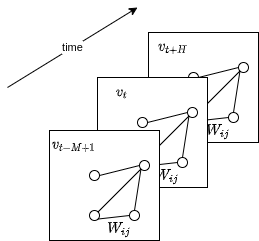
\includegraphics{./images/base.png}
  \centering
  \caption{
نمایش رابطه \رجوع{eq:base} به صورت شهودی.
گراف مسیر یکسان است و هر دیاگرام نشان‌دهنده‌ی سرعت ترافیک در گره‌های این گراف در یک لحظه متفاوت است.
}
  \label{fig:base}
\end{figure}

بدیهی است تغییر سرعت ترافیک در یک گره‌ی گراف می‌تواند باعث تغییر سرعت ترافیک در گره‌های مجاور شود و هر چه فاصله‌ی دو گره از یک دیگر کم تر باشد این اثرگذاری قوی‌تر است.
برای نمایش این عامل به صورت کمی از ماتریس $W$ استفاده می‌کنیم، ابعاد این ماتریس به صورت $n \times n$ است که $n$ برابر تعداد گره‌های گراف است و هر مقدار داخل این ماتریس تابعی از فاصله‌ی بین دو گره متناظر است که مقدار آن با کاهش این فاصله بیشتر می‌شود.

در شکل \رجوع{fig:base} $W_{i,j}$ مقدار ماتریس $W$ در خانه‌ی $i$ و $j$ است که نشان دهنده‌ی میزان ارتباط مکانی و همبستگی بین گره‌های $i$ و $j$ می‌باشد.
در این مثال گره‌های $i$ و $j$ همان میادین یاد شده هستند و $W_{i,j}$ با توجه به فاصله‌ی مکانی این دو میدان نشان می‌دهد که
به طور مثال اگر سرعت ترافیک در میدان فاطمی کاهش پیدا کند این موضوع چقدر می‌تواند بر روی سرعت ترافیک در میدان فلسطین تاثیر بگذارد.
در این پروژه از رابطه‌ \رجوع{eq:distance} برای بدست آوردن خانه‌های ماتریس $W$ استفاده می‌کنیم \مرجع{1709.04875}:

\begin{equation}
  W_{i,j} = \left\{
    \begin{array}{ll}
      \exp(-\frac{d^{2}_{ij}}{\sigma^{2}}) & , i \neq j \quad and \quad \exp(-\frac{d^{2}_{ij}}{\sigma^{2}}) \geq \epsilon \\
      0 & , otherwise. \\
    \end{array}\right.
  \label{eq:distance}
\end{equation}

\begin{table}[h]
  \centering
  \caption{توضیح پارامترهای رابطه \رجوع{eq:distance}}
  \begin{tabular}{|c|p{0.5\textwidth}|}
    \hline
    $W_{ij}$ & میزان ارتباط مکانی بین گره‌های $i$ و $j$ \\
    \hline
    $d_{ij}$ & فاصله ی مکانی بین گره‌های $i$ و $j$ \\
    \hline
    $\sigma$, $\epsilon$ & پارامترهای ثابت برای کنترل میزان تنک\پانویس{Sparsity} بودن ماتریس $W$ \\
    \hline
  \end{tabular}
  \label{tbl:distance}
\end{table}

در مثال ما فاصله بین میدان‌های فاطمی و فلسطین برابر $1.7$ کیلومتر است.
هرچه $\epsilon$ را افزایش دهیم باعث می‌شود تنها ارتباطات قوی‌تر را به حساب بیاوریم و ماتریس تنک‌تر می‌شود
همچنین هرچه $\sigma$ را کاهش دهیم عددی که به عنوان میزان ارتباط محاسبه می‌کنیم کاهش یافته و ماتریس تنک‌تر می‌شود.

با توجه به توضیحات بالا برنامه توسعه‌یافته‌ی نهایی بر اساس این مدل برای عملکرد به دو فایل ورودی احتیاج دارد که اطلاعات درج شده در شکل \رجوع{fig:blackbox} را در اختیار برنامه قرار دهند.
فایل اول شامل ماتریس $W$ است که پیشتر توضیح داده شد و گراف یا به عبارتی وزن یال‌ها را شرح می‌دهد،
فایل دیگر شامل سرعت ترافیک در نودهای این گراف در بازه‌های زمانی متوالی قرار می‌گیرد $(V_{t}, \ldots, V_{t-M+1})$.
در خروجی، سرعت ترافیک پیش‌بینی شده در نودها در قدم‌های زمانی بعدی برگردانده می‌شود $\hat{V}$.
در مثال ما فایل‌های ذکر شده فرمتی مانند جدول \رجوع{tbl:speed-example} و \رجوع{tbl:distance-example} دارند البته اعداد زیر به صورت تصادفی و فرضی هستند.

\begin{figure}
  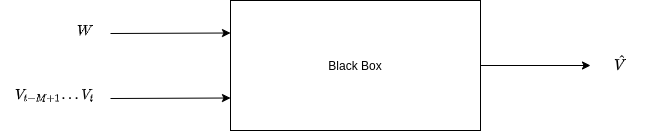
\includegraphics[height=3cm]{./images/blackbox.png}
  \centering
  \caption{
در یک نگاه سطح بالا برنامه با دانستن گراف و سرعت ترافیک در گره‌های این گراف در $M$ واحد زمانی گذشته سرعت ترافیک در $H$ واحد زمانی بعدی را تخمین زده و برمی‌گرداند.
  }
  \label{fig:blackbox}
\end{figure}

\شروع{لوح}[h]
\شرح{مثالی از فرمت فایل ورودی برنامه که شامل سرعت ترافیک در میادین فلسطین و فاطمی در سه قدم زمانی است.}
\تنظیم‌ازوسط
\برچسب{tbl:speed-example}
\شروع{جدول}{|c|c|c|c|}
\خط‌پر
۲ بعد از ظهر & ۱:۵۵ بعد از ظهر & ۱:۵۰ بعد از ظهر & \\
\خط‌پر
۳۶ کیلومتر بر ساعت & ۳۲ کیلومتر بر ساعت & ۴۰ کیلومتر بر ساعت & میدان فلسطین \\
\خط‌پر
۱۷ کیلومتر بر ساعت & ۲۷ کیلومتر بر ساعت & ۱۰ کیلومتر بر ساعت & میدان فاطمی \\
\خط‌پر
\پایان{جدول}
\پایان{لوح}

\شروع{لوح}[h]
\شرح{مثالی از فرمت فایل ورودی برنامه که شامل وزن یالها برای نشان دادن میزان ارتباط مکانی است.}
\تنظیم‌ازوسط
\برچسب{tbl:distance-example}
\شروع{جدول}{|c|c|c|}
\خط‌پر
میدان فاطمی & میدان فلسطین & \\
\خط‌پر
۳۱۶ & ۰ & میدان فلسطین \\
\خط‌پر
۰ & ۳۱۶ & میدان فاطمی \\
\خط‌پر
\پایان{جدول}
\پایان{لوح}


برای سادگی گراف را بدون جهت در نظر می‌گیریم و در نتیجه $W$ ماتریسی متقارن است.

برنامه برای آنکه بتواند هم ارتباطات مکانی و هم ارتباطات زمانی را یاد بگیرد باید از بلوک‌هایی تشکیل شده باشد که هر دو نوع لایه پیچشی زمانی و مکانی را در خود داشته باشند.
همانطور که در شکل \رجوع{fig:blocks} نشان داده شده است، ساختار برنامه از دو بلوک پیچشی زمانی-مکانی و یک لایه‌ی خروجی کاملا متصل در انتها تشکیل شده است.

\begin{figure}
  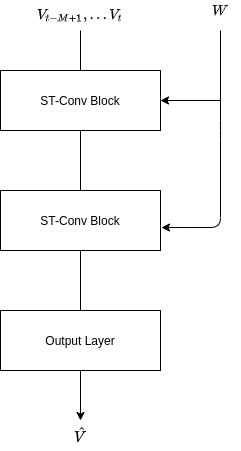
\includegraphics[height=8cm]{./images/blocks.png}
  \centering
  \caption{
شبکه‌ی پیچشی زمانی-مکانی بر روی گراف \مرجع{1709.04875}
  }
  \label{fig:blocks}
\end{figure}

هر بلوک پیچشی زمانی-مکانی که در شکل \رجوع{fig:inner-blocks} نشان داده شده است از دو لایه‌ی پیچشی زمانی تشکیل شده است که در ورودی و خروجی قرار گرفته‌اند
و یک لایه‌ی پیچش مکانی گراف مانند پلی بین آن دو قرار گرفته است، که می‌تواند با سرعت خوبی اطلاعات مکانی را پس از اعمال پیچش روی گراف
به پیچش‌های زمانی انتشار دهد.

\begin{figure}
  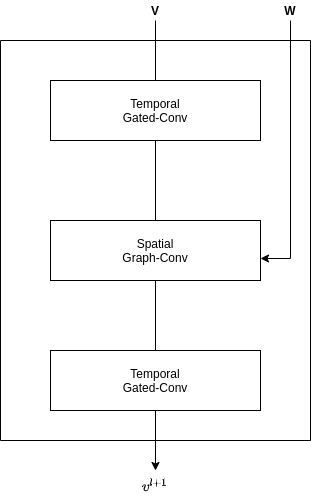
\includegraphics[height=8cm]{./images/inner-blocks.png}
  \centering
  \caption{
ساختار بلوک پیچشی زمانی-مکانی. گراف مسیرها تنها در لایه‌ی پیچش مکانی گراف استفاده می‌شود. \مرجع{1709.04875}
  }
  \label{fig:inner-blocks}
\end{figure}

در این پروژه برای استخراج ویژگی‌های مکانی از پیچش روی گراف استفاده می‌کنیم و بدیهی است پیچش استاندارد که معمولا
در بحث پردازش تصویر روی تصاویر اعمال می‌کنیم در این مساله قابل استفاده نیست
چرا که در پردازش تصویر پیچش عملا کار الگویابی\پانویس{Pattern Matching} را انجام می‌دهد اما در گراف که رئوس جای مشخصی ندارد
و راس‌های یک گراف را می‌توان به صورت‌های مختلفی
شماره‌گذاری کرد نمی‌توان از پیچش انتظار الگویابی داشت.
و باید از مدل عمومی‌تری استفاده کنیم.

در پردازش تصویر از کرنل‌هایی مانند شکل \رجوع{fig:2d-convolution} استفاده می‌شود. تمامی خانه‌ها همواره در جای مشخص خود و با ترتیب ثابت قرار گرفته‌اند
برای مثال خانه‌ی $j3$ همیشه در گوشه بالا قرار گرفته است.

\begin{figure}
  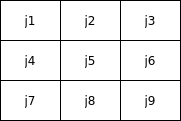
\includegraphics[]{./images/2d-convolution.png}
  \centering
  \caption{کرنل پیچش دو بعدی}
  \label{fig:2d-convolution}
\end{figure}

می‌خواهیم کرنل شکل \رجوع{fig:graph-convolution-kernel}
به گراف شکل \رجوع{fig:graph-convolution-graph} اعمال کنیم و واضح است که یک نام‌گذاری با ترتیب یکسان برای گراف و کرنل وجود ندارد.


\begin{figure}
  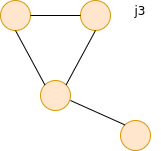
\includegraphics[]{./images/graph-convolution-kernel.png}
  \centering
  \caption{کرنل پیچش گراف}
  \label{fig:graph-convolution-kernel}
\end{figure}

\begin{figure}
  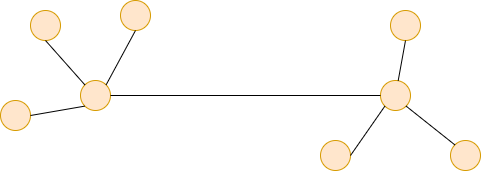
\includegraphics[]{./images/graph-convolution-graph.png}
  \centering
  \caption{گراف مقصد پیچش گراف}
  \label{fig:graph-convolution-graph}
\end{figure}

در این پژوهش از پیچش طیفی روی گراف‌\پانویس{Spectral Graph Convolution} استفاده می‌کنیم. \مرجع{1312.6203}

با استفاده از رابطه \رجوع{eq:convolution} می‌توانیم پیچش روی گراف را انجام دهیم تا الگوها و ویژگی‌های با معنی را در دامنه‌ی فضا پیدا کنیم.

\begin{equation}
  \Theta *_{g} \chi = \Theta(L)\chi = \Theta(U \Lambda U^{T})\chi = U\Theta(\Lambda)U^{T}\chi
  \label{eq:convolution}
\end{equation}

\begin{table}[h]
  \centering
  \caption{توضیح پارامترهای رابطه \رجوع{eq:convolution}}
  \begin{tabular}{|c|p{0.5\textwidth}|}
    \hline
    $*_{g}$ & عامل پیچش مکانی روی گراف \\
    \hline
    $\chi$ & سیگنال گراف که در این مدل خروجی لایه‌ی پیچش زمانی اول است \\
    \hline
    $\Theta$ & کرنل \\
    \hline
    $L$ & ماتریس لاپلاسین نرمال شده‌ی گراف \\
    \hline
    $U$ & ماتریس بردار ویژه‌های ماتریس $L$ \\
    \hline
    $\Lambda$ & ماتریس قطری مقدار ویژه‌های ماتریس $L$ \\
    \hline
  \end{tabular}
  \label{tbl:distance}
\end{table}

در مثال ذکر شده اگر محاسبات را انجام دهیم، خواهیم داشت:

\[
U = \left(
  \begin{array}{cc}
  1 & -1 \\
  1 & 1 \\
  \end{array}
\right),
\Lambda = \left(
  \begin{array}{cc}
  0 & 0 \\
  0 & 2 \\
  \end{array}
\right),
L = \left(
  \begin{array}{cc}
  1 & -1 \\
  -1 & 1 \\
  \end{array}
\right)
\]

در نظر داشته باشید که المان‌های ماتریس $\Theta$ در ابتدا به صورت تصادفی انتخاب می‌شوند.

پیچیدگی زمانی این رابطه $O(n^{2})$ است که بسیار سنگین است، برای سبک شدن محاسبات باید از یک تخمین به جای استفاده مستقیم از این رابطه بهره ببریم.
در این پروژه از تخمین چند جمله‌ای چبیشف\پانویس{Chebyshev} استفاده می‌کنیم.

برای متمرکز و محلی کردن فیلتر و کاهش تعداد پارامترها، می‌توان کرنل $\Theta$ را به یک چند جمله‌ای از $\varLambda$ محدود کرد.

\[
  \Theta(\varLambda) = \sum_{k=1}^{k-1}\Theta_{k}\varLambda^{k}
\]

$k$ اندازه کرنل در پیچش گراف است که شعاع بیشینه پیچش از یک گره مرکزی را مشخص می‌کند. از چند جمله‌ای چبیشف $T_{k}(x)$ استفاده می‌کنیم تا
کرنل‌ها را به صورت انبساطی کوتاه شده از مرتبه‌ی $k-1$ تخمین بزنیم.

 از چند جمله‌ای چبیشف
( $T_{k}(x)$ )
 استفاده می‌کنیم تا کرنل‌ها را به صورت انبساطی کوتاه شده از مرتبه‌ی
 $k-1$
 تخمین بزنیم.

\[
  \Theta(\varLambda) \approx \sum_{k=1}^{k-1}\Theta_{k}T_{k}(\widetilde{\varLambda})
\]
\[
  \widetilde{\varLambda} = \frac{2\varLambda}{\lambda_{\max}} - I_{n}
\]

% \begin{table}[h]
%   \centering
%   \caption{توضیح پارامترهای رابطه \رجوع{eq:convolution}}
%   \begin{tabular}{|c|p{0.5\textwidth}|}
%     \hline
%     $\Lambda$ & ماتریس قطری مقدار ویژه‌های ماتریس $L$ \\
%     \hline
%     $\lambda_{\max}$
%     & بزرگ‌ترین مقدار ویژه‌ی ماتریس لاپلاسین \\
%     \hline
%     $\Theta$ & کرنل \\
%     \hline
%     $L$ & ماتریس لاپلاسین نرمال شده‌ی گراف \\
%     \hline
%     $U$ & ماتریس بردار ویژه‌های ماتریس $L$ \\
%     \hline
%     $\widetilde{\varLambda}$
%     & $\varLambda$ اسکیل شده \\
%     \hline
%   \end{tabular}
%   \label{tbl:distance}
% \end{table}

حال می‌توانیم پیچش روی گراف را اینگونه بازنویسی کنیم:

\begin{equation}
  \Theta \ast_{g} x = \Theta(L)x \approx \sum_{k=0}^{k-1} \Theta_{k} T_{k}(\widetilde{L})x
  \label{eq:approx-convolution}
\end{equation}

$T_{k}(\widetilde{L} \in R^{n \times n})$ چند جمله‌ای چبیشف از مرتبه‌ی $k$ است که به وسیله‌ی لاپلاسین اسکیل شده محاسبه می‌شود.

\[
  \widetilde{L} = \frac{2\widetilde{L}}{\lambda_{\max}} - I_{n}
\]

از تقریب چند جمله‌ای استفاده می‌کنیم و به طور بازگشتی $k$ پیچش‌های محلی را محاسبه می‌کنیم. اینگونه می‌توانیم رابطه‌ی \رجوع{eq:convolution}
را با رابطه‌ی \رجوع{eq:approx-convolution} تخمین بزنیم و پیچیدگی محاسباتی را از $O(n^{2})$ به $O(k|\epsilon|)$
کاهش دهیم.

\زیرقسمت{تعمیم دادن کانولوشن روی گراف}
\پاراگراف{}
عامل کانولوشن بر روی گراف (
$*_g$
)که پیشتر تعریف کردیم تنها می توانست بر روی یک
$x \in R^n$
اعمال شود. می توانیم آن را تعمیم دهیم به طوری که بر روی تنسورهای چندبعدی نیز قابل اعمال باشد. برای سیگنالی با
$c_i$
کانال (
$X \in R^{n*c_i}$
)
کانولوشن روی گراف را می توان اینگونه تعمیم داد

\begin{equation}
y_i = \sum_{i=1}^{C_i} \Theta _{i,j}(L)x_i \in R^n , 1 <= j <= C_o
    \label{eq:graph-convolution-generalization}
\end{equation}

\begin{table}[h]
  \centering
  \caption{توضیح پارامترهای رابطه \رجوع{eq:graph-convolution-generalization}}
  \begin{tabular}{|c|p{0.5\textwidth}|}
    \hline
    $C_i$ & سایز ورودی نگاشت ویژگی\پانویس{feature map} \\
    \hline
    $C_o$ & سایز خروجی نگاشت ویژگی \\
    \hline
    $\Theta_{i,j} \in R^k$ & بردارهای ضرایب چبیشف که تعداد آن‌ها
    $C_i * C_o$
    می‌شود.\\
    \hline
  \end{tabular}
  \label{tbl:distance}
\end{table}

\پاراگراف{}
کانولوشن بر روی گراف برای متغیرهای دو بعدی به صورت
$\Theta *_g X$
نشان داده می‌شود (
$\Theta \in R^{K*C_i*C_o}$
. در این پروژه برای پیش‌بینی ترافیک ورودی از
$M$
صفحه تشکیل شده‌است که هر صفحه گراف مسیرها را در یک گام زمانی نشان می‌دهد ( شکل
\رجوع{fig:base}
).
هر صفحه مربوط به گام زمانی
$t$
را می توان به صورت یک ماتریس دید که ستون
$i$
ام آن مقدار
$C_i$
بعدی از سرعت ترافیک در گره
$i$
ام از گراف است (
$X \in R^{n * C_i}$
)

\پاراگراف{}
در مسائل سری زمانی، شبکه‌های عصبی بازگشتی بسیار رایج‌اند اما در مسایل ترافیک استفاده از این شبکه‌ها بسیار زمان‌بر است.
همچنین در ترافیک تغییرات به صورت پویا می‌باشند که این شبکه دیر به این تغییرات جواب می‌دهد،
در طرف دیگر شبکه های عصبی پیچشی به سرعت آموزش داده می‌شوند و ساختار ساده‌ای دارند، در نتیجه برای استخراج ویژگی‌های زمانی در این پروژه با الهام از
\مرجع{1409.3215} از ساختارهای کاملا پیچشی بر روی محور زمان استفاده می‌کنیم تا بتوانیم رفتار پویای سرعت ترافیک را دنبال کنیم.

\begin{figure}
  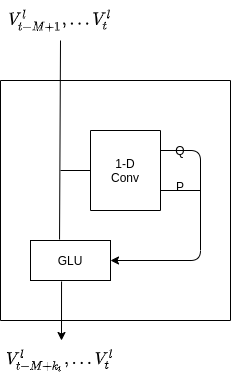
\includegraphics[height=8cm]{./images/time-conv.png}
  \centering
  \caption{
ساختار لایه‌ی کانولوشنی زمانی \مرجع{1709.04875}
  }
  \label{fig:time-conv}
\end{figure}

\پاراگراف{}
شکل \رجوع{fig:time-conv} لایه‌ی پیچشی زمانی را نشان می‌دهد که شامل یک پیچش علّی یک بعدی\پانویس{1-D casual convolution}
با یک فیلتر به عرض  $k_{t}$ است که پس از آن یک \متن‌لاتین{Gated Linear Unit} قرار دارد.
برای هر گره در گراف $g$ پیچش زمانی بر روی تمامی $K_{t}$ همسایه‌ی ورودی اعمال می‌شود.
در این پیچش لایه گذاری\پانویس{padding} وجود ندارد‌‌، در نتیجه، پیچش در هر مرتبه باعث کوتاه‌تر شدن توالی‌ها به اندازه‌ی $K_{t}-1$ می‌شود.
با این توضیحات می‌توانیم رابطه‌ی \رجوع{eq:time-conv} را بیان کنیم.

\begin{equation}
  \Gamma *_{\tau} Y = P \odot \sigma (Q) \in R^{M-K_{t}+1 \times C_{O}}
  \label{eq:time-conv}
\end{equation}

\begin{table}[h]
  \centering
  \caption{توضیح پارامترهای رابطه \رجوع{eq:time-conv}}
  \begin{tabular}{|c|p{0.5\textwidth}|}
    \hline
    $*_{g}$ & عامل پیچش زمانی \\
    \hline
    $Y$ & سرعت ترافیک در گره‌های مختلف گراف در گام‌های زمانی گذشته \\
    \hline
    $\Gamma$ & کرنل پیچش که المان‌های آن در ابتدا به صورت تصادفی انتخاب می‌شوند. \\
    \hline
    $P$, $Q$ & پس از آنکه با استفاده از کرنل $\Gamma$ یک پیچش روی $Y$ اعمال کردیم خروجی را برحسب سایز کانال خروجی لایه به دو نیمه‌ی مساوی تقسیم می‌کنیم که یکی $P$ و دیگری را $Q$ می‌نامیم. \\
    \hline
    $\odot$ & نمایشگر عملیات ضرب درایه‌ای \\
    \hline
    $M$ & تعداد گام‌های زمانی استفاده شده برای آموزش \\
    \hline
    $K_{t}$ & سایز کرنل \\
    \hline
    $C_{O}$ & سایز کانال خروجی \\
    \hline
  \end{tabular}
  \label{tbl:distance}
\end{table}

 $P$ و $Q$ پس از محاسبه به عنوان ورودی به \متن‌لاتین{Gated Linear Unit} داده می‌شوند، این واحد باعث غیرخطی شدن محاسبات این لایه می‌شود.

ورودی $Y$ چهار بعدی است، بُعد اول برابر تعداد کل داده‌هایی است که در اختیار داریم، بُعد دوم برابر
تعداد گام‌های گذشته است، که قصد داریم برای پیش‌بینی استفاده کنیم،
بُعد سوم برابر تعداد گره‌های گراف و در نهایت بُعد آخر سایز کانال ورودی است.
در مثالی که با آن پیش می‌رویم تعداد کل داده‌ها سه، تعداد گام‌های زمانی گذشته مورد استفاده برای پیش‌بینی مدل برابر دو،
تعداد گره‌های گراف برابر دو و سایز کانال ورودی برابر یک است، در نتیجه ابعاد $Y$ به صورت $ 3 \times 2 \times 2 \times 1 $ در میاید.

همانطور که پیش‌تر اشاره شد در این پیچش لایه‌گذاری وجود ندارد در نتیجه ابعاد خروجی این لایه مانند ابعاد ورودی است به جز بعد دوم
که پس اعمال پیچش به اندازه‌ی $K_{t}-1$ کاهش میابد. حال اگر عرض $K_{t}$ را در مثالمان برابر ۲ در نظر بگیریم
بعد دوم ورودی به اندازه‌ی ۱ واحد کوچکتر و برابر با ۱ می‌گردد.

از آنجایی که مقادیر کرنل $\Gamma$ تصادفی می‌باشند، ادامه مثال ارزش افزوده‌ای نداشته بنابراین به آوردن مثال تا به این نقطه بسنده می‌کنیم.

در نهایت بلوک‌های پیچش زمانی-مکانی از رابطه \رجوع{eq:blocks} پیروی می‌کنند که در آن $L_{0}$ و $L_{1}$ به ترتیب کرنل‌ لایه‌های پیچشی زمانی پایینی و بالایی و $\Theta$ کرنل پیچش مکانی روی گراف می‌باشد.

\begin{equation}
v^{{l+1}} = \Gamma^{l}_{1} *_{\tau} ReLU( \Theta^{l} *_{g} (\Gamma_{0}^{l} *_{\tau} v^{l}) )
  \label{eq:blocks}
\end{equation}

بعد از روی هم قرار دادن دو بلوک پیچش زمانی-مکانی یک لایه‌ی کاملا متصل به عنوان لایه‌ی خروجی در انتها قرار می‌دهیم (مطابق شکل \رجوع{fig:blocks}).

در این پروژه قصد داریم سرعت ترافیک در \متن‌لاتین{H} قدم زمانی بعدی را پیش‌بینی کنیم در مسایلی از این قبیل از چهار روش متفاوت می‌توانیم عمل کنیم:
۱. از آن جایی که در پروژه از شبکه‌های عصبی استفاده می‌کنیم و این مدل‌ها می‌توانند چندین خروجی داشته باشند، می‌توانیم در لایه‌ی آخر مدل شبکه‌ی عصبی خود به تعداد \متن‌لاتین{H} نورون قرار دهیم و با یک مدل سرعت ترافیک در \متن‌لاتین{H} قدم زمانی بعدی را پیش‌بینی کنیم.
۲. می توانیم از روش مستقیم \پانویس{direct} استفاده کرده و برای هر خروجی یک مدل مجزا آموزش دهیم.
۳. می توانیم از روش بازگشتی \پانویس{recursive} استفاده کنیم به طوری که خروجی مدل به عنوان ورودی به خود مدل داده می‌شود.
۴. می توانیم از روش مستقیم-بازگشتی \پانویس{direct-recursive} استفاده کنیم در این روش مدل مجزایی برای هر خروجی آموزش داده می‌شود و همچنین خروجی یک مدل به عنوان ورودی به مدل بعدی داده می‌شود

در این پروژه \متن‌لاتین{‌H} یک ابرپارامتر است و قصد نداریم آن را ثابت فرض کنیم به هین دلیل روش اول و همچنین روش مستقیم برای ما مناسب نیست و از روش بازگشتی استفاده می‌کنیم. لایه‌ی خروجی تنها یک کانال دارد و در نتیجه سرعت رافیک را تنها برای یک گام بعدی می توان پیش‌بینی کرد در صورتی که در تعریف مساله بیان کرده بودیم قصد داریم این ویژگی را برای،
$H$
قدم بعدی پیش‌بینی کنیم بدین منظور از روش پنجره‌ی لغزان\پانویس{window-based}
استفاده می‌کنیم به این صورت که با استفاده از پنجره‌ای به طول
$M$
از
$M$
داده‌ی قبلی استفاده می‌کنیم تا سرعت ترافیک در گام بعدی را پیش‌بینی کنیم سپس این پنجره را یک واحد حرکت می دهیم به طوری که پیش‌بینی مدل در مرحله‌ی قبل حال به عنوان آخرین داده در این پنجره قرار می‌گیرد و برای پیش ‌بینی سرعت در گام بعدی مورد استفاده قرار می‌گیرد، این روند را تا
$H$
مرحله ادامه می دهیم. بدیهی است پیشی‌بینی مدل برای گام‌های ابتدایی دقیق‌تر از گام‌های انتهایی است.


\begin{figure}
  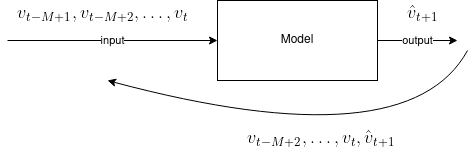
\includegraphics[height=8cm]{./images/recursive.png}
  \centering
  \caption{
روش بازگشتی در پیش‌بینی چند گام آینده }
  \label{fig:blocks}
\end{figure}


\قسمت{ابزارها و امکانات مورد نیاز}
مرتبه زمانی روش پیچش روی گراف به این دلیل که امکان استفاده از تبدیل سریع فوریه\پانویس{FFT} وجود ندارد،
\[
O(n^{2})
\]
می‌باشد و اعمال این روش بدون داشتن تجهیزات گران قیمتی مانند پردازنده‌های گرافیکی زمان قابل توجهی است. حداقل امکانات مورد نیاز برای اجرای این پروژه عبارت اند از:

\begin{latin}\begin{itemize}
\item CPU: Intel(R) Xeon(R) CPU E5-2620 v4 @ 2.10GHz
\item GPU: NVIDIA GeForce GTX 1080
\end{itemize}\end{latin}

\قسمت{توضیح دیتاست}
مدل را دوبار به وسیله ی دو داده‌گان متفاوت آموزش دادیم.

\زیرقسمت{داده‌گان \متن‌لاتین{PeMSD7}}

این دیتاست توسط دوربین‌های سرعت‌سنجی که در نقاط مختلف قرار می‌گیرند جمع آوری شده‌اند. محل استقرار این دوربین‌ها ثابت است و کار ما در ساختن ماتریس فاصله بسیار ساده می کند همچنین سرعتی که این دوربین‌ها گزارش می‌دهند بسیار قابل اعتماد است و دیتاستی که با آن کار کردیم نیز داده‌ی پرت و یا گمشده‌ی کمی داشت و همانظور که در جدول \رجوع{} مشاهده می‌کنید مدل آموزش داده شده با این دیتاست دقت بالایی دارد.

\زیرقسمت{داده‌گان \متن‌لاتین{Snapp}}

این دیتاست توسط سیستم موقعیت‌‌یاب‌جهانی رانندگان جمع‌آوری شده‌است در نتیجه نمی‌توان سرعت ترافیک یک نقطه را پیدا کرد بلکه می‌توان
به طور مثال سرعت ترافیک در یک خیابان را دانست این موضوع ساختن ماتریس فاصله را مشکل می‌کند همچنین داده‌های آن به دلایل متعدی مانند
وجود ساختمان‌های بلند قابل اعتماد نیست. همچنین این داده در ابتدا سرعت ترافیک در یک خیابان نیستند بلکه سیگنال‌های \متن‌لاتین{GPS} رانندگان است. برای آماده کردن داده مراحل زیر انجام شده است.

\شروع{شمارش}

\فقره نوشتن \متن‌لاتین{cron job} برای گرفتن داده‌گان: به علت حجم بالای داده‌گان گرفتن تمام داده‌گان به صورت پشت‌سر‌هم مقدور نبود
در نتیجه \متن‌لاتین{cron job} نوشته شد تا در هر دقیقه تلاش کند و یک \متن‌لاتین{bulk} از دادگان را بگیرد.

\فقره نگاشت نقطه بر نقشه\پانویس{map matching}: سیگنال \متن‌لاتین{GPS} رانندگان به صورت دقیق بر روی خیابان نمی‌افتد و ابتدا باید خیابان مربوط به هر سیگنال \متن‌لاتین{‌GPS} را پیدا کنیم.

\شروع{شکل}
  \درج‌تصویر[height=8cm]{./images/mapMatch.png}
  \تنظیم‌ازوسط
  \شرح{نگاشت نقطه بر نقشه}
  \برچسب{fig:time-conv}
\پایان{شکل}

هر سیگنال \متن‌لاتین{GPS} متعلق به یک خیابان است که خیابان مورد نظر برای ما پنهان است و ما تنها سیگنال را می‌توانیم مشاهده کنیم
از طرفی ما رشته‌ی این سیگنال‌های \متن‌لاتین{GPS} را داریم، در نتیجه می‌توانیم از الگوریتم مدل پنهان مارکوف\پانویس{hidden markov model} \مرجع{Rabiner1986} استفاده کنیم.
برای هر سیگنال می توان $k$ خیابان نزدیک به آن را به عنوان حالت‌های پنهان احتمالی فرض کرد و سپس احتمالات انتشار و انتقال را به‌دست‌آورد.

\شروع{شکل}
  \درج‌تصویر[height=8cm]{./images/hmm.png}
  \تنظیم‌ازوسط
  \شرح{مدل پنهان مارکوف}
  \برچسب{fig:time-conv}
\پایان{شکل}

حال با استفاده از الگوریتم ویتربی\پانویس{viterbi} می توانیم محتمل‌ترین رشته و در نتیجه محتمل‌ترین نگاشت را پیدا کنیم.
پس از اتمام عملیات نگاشت می‌توانیم سرعت حرکت راننده، جهت حرکت او و شماره‌ی مرجع خیابان \پانویس{Road Segment ID} را پیدا کنیم.

\فقره محاسبه‌ی سرعت بر اساس سیگنال‌های \متن‌لاتین{GPS}: یکی از اطلاعاتی که سیگنال \متن‌لاتین{GPS} در اختیار ما قرار می‌دهد سرعت است اما این سرعت به صورت لحظه‌ای است و دارای خطای بسیار زیادی است به همین دلیل خود به محاسبه‌ی سرعت می‌پردازیم. پس از مرحله‌ی قبل که رشته‌ی \متن‌لاتین{GPS}های پشت‌سر‌هم به دست آمدند از تقسیم فاصله‌ی کروی دو سیگنال پشت‌سر‌هم بر اختلاف زمانی رخ دادن آن‌ها سرعت محاسبه می‌شود.

\فقره تمیز کردن دادگان: دادگان \متن‌لاتین{GPS} رانندگان دارای صفر و داده‌های پرت بسیاری است و نیاز دارد تا به دقت پیش‌پردازش شود. به طور مثال باید چک شود که دادگان راننده‌ّهایی که در حال سفر نیستند حذف شود.

\پایان{شمارش}

\فصل{ارزیابی}

در نهایت به منظور ارزیابی پروژه از دو مجموعه داده‌ی ترافیکی واقعی \متن‌لاتین{PeMSD7} و اسنپ! استفاده می‌کنیم.
برای مقایسه‌ی عملکرد این روش با روش‌های دیگر از معیارهای میانگین مطلق خطا\پانویس{MAE}، میانگین مطلق درصد خطا\پانویس{MAPE} و جذر میانگین مربعات خطا\پانویس{RMSE} استفاده می‌کنیم.
این روش را با روش‌های پایه‌ی شبکه‌ی عصبی پیش‌خور\پانویس{Feed-Forward Neural Network}، مدل خودهمبسته میانگین متحرک و حافظه‌ی کوتاه مدت ماندگار کاملا متصل\پانویس{Full-Connected LSTM} \مرجع{1409.3215} مقایسه خواهیم کرد.

\قسمت{\متن‌لاتین{PeMSD7}}

این مجموعه داده تمیز شده است و آماده‌ی دادن به مدل است. اجرای آموزش با کلاستر لینوکس(پردازنده: \متن‌لاتین{Intel(R) C}، کارت گرافیک: \متن‌لاتین{NVIDIA Ge}) انجام شده است.
تعداد ایپاک ها برابر ۵۰ قرار داده شد و در کل حدود ۳۸ ساعت زمان برد.
در حین آموزش مدل به دلیل قطعی برق تمامی اطلاعات را از دست دادیم به همین جهت پس از هر ایپاک یک بار مدل را ذخیره می‌کنیم تا در صورت رخ دادن اتفاقی مشابه بتوانیم آموزش را از همان قسمتی که دچار مشکل شده بود ادامه دهیم. نتایج اجرا در زیر آورده شده است:

\begin{table}[h]
  \centering
  \caption{نتایج اجرا بر روی مجموعه داده‌ی \متن‌لاتین{PeMSD7}}
  \begin{tabular}{|c|c|c|c|}
    \خط‌پر
    مدل & \متن‌لاتین{MAE} & \متن‌لاتین{MAPE (\%)} & \متن‌لاتین{RMSE}
    \خط‌پر
    \متن‌لاتین{ARIMA}
    \خط‌پر
  \end{tabular}
\end{table}

\قسمت{اسنپ!}

آموزش مدل بر روی مجموعه داده‌ی اسنپ انجام شده است. تعداد ایپاک ها برابر ۵۰ قرار داده شد و در کل حدود ۲۲ ساعت زمان برد. نتایج اجرا در زیر آورده شده است:

\begin{table}[h]
  \centering
  \caption{نتایج اجرا بر روی مجموعه داده‌ی اسنپ!}
  \begin{tabular}{|c|c|c|c|}
    \خط‌پر
    مدل & \متن‌لاتین{MAE} & \متن‌لاتین{MAPE (\%)} & \متن‌لاتین{RMSE}
    \خط‌پر
    \متن‌لاتین{ARIMA}
    \خط‌پر
  \end{tabular}
\end{table}

به طور مثال برای قسمتی از خیابان ولیعصر که در شکل؟؟؟؟؟؟؟؟؟؟ نشان داده شده‌است، نمودار سرعت و سرعت پیش بینی شده را رسم می‌کنیم

\شروع{شکل}
  \درج‌تصویر[height=8cm]{./images/valiasr_osm.jpg}
  \تنظیم‌ازوسط
  \شرح{سیستم \متن‌لاتین{sharedstreet} در برابر سیستم اطلاعات جغرافیایی}
  \برچسب{fig:time-conv}
\پایان{شکل}

 داخل این \متن‌لاتین{osm way} شش \متن‌لاتین{SharedStreet} وجود دارد. برای \متن‌لاتین{SharedStreet} نشان داده شده در شکل؟؟؟؟؟؟؟؟؟ اطلاعات را بر روی نمودار می‌بریم.

\شروع{شکل}
  \درج‌تصویر[height=8cm]{./images/valiasr_shared.png}
  \تنظیم‌ازوسط
  \شرح{سیستم \متن‌لاتین{sharedstreet} در برابر سیستم اطلاعات جغرافیایی}
  \برچسب{fig:time-conv}
\پایان{شکل}

از آن جایی که اکثر سفرهای این شرکت در بازه‌ی زمانی جهار و نیم تا هفت بعد از ظهر انجام می‌شود و تخمین زمان سفر در این بازه از اهمیت بالایی برخوردار است ما نیز نمودار زیر را در این بازه برای روز شنبه، شانزدهم بهمن ۱۴۰۰ رسم می‌کنیم


\شروع{شکل}
  \درج‌تصویر[height=8cm]{./images/p1.png}
  \تنظیم‌ازوسط
  \شرح{سیستم \متن‌لاتین{sharedstreet} در برابر سیستم اطلاعات جغرافیایی}
  \برچسب{fig:p1}
\پایان{شکل}


\شروع{شکل}
  \درج‌تصویر[height=8cm]{./images/p2.png}
  \تنظیم‌ازوسط
  \شرح{سیستم \متن‌لاتین{sharedstreet} در برابر سیستم اطلاعات جغرافیایی}
  \برچسب{fig:p2}
\پایان{شکل}


\شروع{شکل}
  \درج‌تصویر[height=8cm]{./images/p3.png}
  \تنظیم‌ازوسط
  \شرح{سیستم \متن‌لاتین{sharedstreet} در برابر سیستم اطلاعات جغرافیایی}
  \برچسب{fig:p3}
\پایان{شکل}


\شروع{شکل}
  \درج‌تصویر[height=8cm]{./images/p4.png}
  \تنظیم‌ازوسط
  \شرح{سیستم \متن‌لاتین{sharedstreet} در برابر سیستم اطلاعات جغرافیایی}
  \برچسب{fig:p4}
\پایان{شکل}



\قسمت{خلاصه}

ارزیابی مدل ارائه شده بر روی دو مجموعه داده \متن‌لاتین{PeMSD7} و اسنپ انجام و نتیجه گزارش شد. ارزیابی این مدل بر روی مجموعه داده‌ی اسنپ نیازمند مراحل بسیاری برای تبدیل \متن‌لاتین{GPS} ها به سرعت بود که همگی در این بخش توضیح داده شدند.

\فصل{نتیجه‌گیری و کارهای آینده}


%--------------------------------------------------------------------------appendix( مراجع و پیوست ها)
\chapterfont{\vspace*{-2em}\centering\LARGE}%

\appendix
\setLTRbibitems{}
\bibliographystyle{ieeetr}
\bibliography{references}
% \chapter*{‌پیوست}
\markboth{پیوست}{}
\addcontentsline{toc}{chapter}{پیوست}
موضوعات مرتبط با متن گزارش پایان نامه كه در يكی از گروه‌های زير قرار می‌گيرد، در بخش پيوست‌ها آورده شوند:
\begin{enumerate}
\item  اثبات های رياضی يا عمليات رياضی طولانی‌.‌
\item داده و اطلاعات نمونه (های) مورد مطالعه (\lr{Case Study}) چنانچه طولانی باشد‌.‌
\item نتايج كارهای ديگران چنانچه نياز به تفصيل باشد‌.‌
\item مجموعه تعاريف متغيرها و پارامترها، چنانچه طولانی بوده و در متن به انجام نرسيده باشد‌.‌
\end{enumerate}
% براي شماره‌گذاري روابط، جداول و اشكال موجود در پيوست‌ از ساختار متفاوتي نسبت به متن اصلي استفاده مي‌شود كه در زير به‌عنوان نمونه نمايش داده شده‌است. 
% \begin{equation}
%F=ma
%\end{equation}
\section*{کد میپل }
\begin{latin}
\begin{verbatim}

with(DifferentialGeometry):
with(Tensor):
DGsetup([x, y, z], M)
																	frame name: M
a := evalDG(D_x)
																	D_x
b := evalDG(-2 y z D_x+2 x D_y/z^3-D_z/z^2)


\end{verbatim}
\end{latin}
%--------------------------------------------------------------------------dictionary(واژه نامه ها)
%اگر مایل به داشتن صفحه واژه‌نامه نیستید، خط زیر را غیر فعال کنید.
\parindent=0pt
%
\chapter*{فهرست اختصارات}
\pagestyle{style9}

\addcontentsline{toc}{chapter}{فهرست اختصارات}
%%%%%%

\abbr{NFV}{Network Function Virtualization}

\abbr{SFC}{Service Function Chaining}

\abbr{SDN}{Software Defined Netwoks}

\abbr{MANO}{Management and Orchestration}

\abbr{VNF}{Virtual Network Function}

\abbr{VNFM}{Virtual Network Function Manager}
%%%%%%
\chapter*{واژه‌نامه}
\pagestyle{style9}
\lhead{\thepage}\rhead{واژه‌نامه}
\addcontentsline{toc}{chapter}{واژه‌نامه}

\englishTOfarsi{Interface}{رابط}

\englishTOfarsi{Application}{کاربرد}

\englishTOfarsi{Optimality Gap}{شکاف بهینه}

\englishTOfarsi{Edge}{یال}

\englishTOfarsi{Node}{گره}

\englishTOfarsi{Virtualization}{مجازی‌سازی}

\englishTOfarsi{Constraint}{محدودیت}

\englishTOfarsi{Heuristic}{مکاشفه‌ای}

\englishTOfarsi{Offline}{برون‌خط}

\englishTOfarsi{Online}{برخط}

\englishTOfarsi{Image}{تصویر}

\englishTOfarsi{Classifier}{دسته‌بند}

\englishTOfarsi{Forwarding}{جلورانی}

\englishTOfarsi{Function}{کارکرد}

\englishTOfarsi{Pod}{غلاف}

\englishTOfarsi{Aggregation}{تجمعی}

\englishTOfarsi{Edge}{لبه}

\englishTOfarsi{Instance}{نمونه}

\englishTOfarsi{Feasible Set}{مجموعه امکان‌پذیر}

\englishTOfarsi{Monitoring}{نظارت}

\englishTOfarsi{Data Center}{مرکز داده}
%--------------------------------------------------------------------------index(نمایه)
%اگر مایل به داشتن صفحه نمایه نیستید، خط زیر را غیر فعال کنید.
\pagestyle{style7}
\printindex
\pagestyle{style7}
%کلمات کلیدی انگلیسی
\latinkeywords{
  transportation, traffic speed prediction, deep neural networks
}
%چکیده انگلیسی

\en-abstract{
  Predicting traffic speed is essential to control and direct it. Due to the complexity and nonlinearity of traffic speed methods
The ancients could not predict traffic well for long and medium time travel. Accurate and immediate forecasting
Traffic speed is an important issue for individuals and organizations providing transportation services and even the government because transportation
Transportation plays an important role in every person's life and is one of the main capabilities in the intelligent transportation system.
Goes. In this project, we try to predict the traffic speed in some by using deep neural networks.
Pay attention to specific points (such as intersections and squares). Using the vast amount of data available today as well
Hardware Advancement We can train deep networks that were not teachable in the past and their high capability
Use in predicting complex issues. In this report, a torsional-spatial graph network is used to predict speed
We used traffic and using the evaluation results of this model on two real data sets, we showed that this network
Deep can effectively understand comprehensive spatio-temporal correlations and thus perform well.
}

%%%%%%%%%%%%%%%%%%%%% کدهای زیر را تغییر ندهید.

\newpage
\thispagestyle{empty}
\begin{latin}
\section*{\LARGE\centering Abstract}

\een-abstract

\vspace*{.5cm}
{\large\textbf{Key Words:}}\par
\vspace*{.5cm}
\elatinkeywords
\end{latin}

% در این فایل، عنوان پایان‌نامه، مشخصات خود و چکیده پایان‌نامه را به انگلیسی، وارد کنید.
%%%%%%%%%%%%%%%%%%%%%%%%%%%%%%%%%%%%
\baselineskip=.6cm
\begin{latin}

\latinfaculty{Department of Computer Engineering}


\latintitle{Design and implementation of traffic forecasting system based on neural networks}


\firstlatinsupervisor{Dr. Reza Safabaksh}

%\secondlatinsupervisor{Second Supervisor}

% \firstlatinadvisor{Dr. }

%\secondlatinadvisor{Second Advisor}

\latinname{Elahe}

\latinsurname{Dastan}

\latinthesisdate{February 2022}

\latinvtitle%
\end{latin}

\end{document}
